\documentclass[12pt]{article}
\usepackage[utf8]{inputenc}
\usepackage[spanish]{babel}
% ---------------------------------------------------
%                       FONT 
% ---------------------------------------------------

%\usepackage{cmbright}                              % Font
\usepackage{bbding}
\decimalpoint
\usepackage[spanish]{babel}
\usepackage{amsmath}
\usepackage{amsthm}
\usepackage{amssymb}
\usepackage{graphicx}
\usepackage[margin=0.9in]{geometry}
\usepackage{fancyhdr}
\usepackage[inline]{enumitem}
\usepackage{float}
\usepackage{cancel}
\usepackage{minted}
\usepackage{bigints}
\usepackage{color}
\usepackage{xcolor}
\usepackage{subfig}
\usepackage{listingsutf8}
\usepackage{algorithm}
\usepackage{tocloft}
\usepackage[none]{hyphenat}
\usepackage{graphicx}
\usepackage{grffile}
\usepackage{tabularx}
\usepackage[nottoc,notlot,notlof]{tocbibind}
\usepackage{times}
\usepackage{color}
\usepackage{multicol}
\definecolor{gray97}{gray}{.97}
\definecolor{gray75}{gray}{.75}
\definecolor{gray45}{gray}{.45}
\renewcommand{\cftsecleader}{\cftdotfill{\cftdotsep}}
\pagestyle{fancy}
\setlength{\headheight}{15pt} 
\lhead{Práctica 4 - Administrador de procesos en Linux y Windows (1)}
\rhead{\thepage}
\lfoot{ESCOM-IPN}
\renewcommand{\footrulewidth}{0.5pt}
\setlength{\parskip}{0.5em}
\newcommand{\ve}[1]{\overrightarrow{#1}}
\newcommand{\abs}[1]{\left\lvert #1 \right\lvert}
\date{26 de febrero de 2017}
\title{Instalación de Netbeans}
\author{Reporte 1}

\definecolor{pblue}{rgb}{0.13,0.13,1}
\definecolor{pgreen}{rgb}{0,0.5,0}
\definecolor{pred}{rgb}{0.9,0,0}
\definecolor{pgrey}{rgb}{0.46,0.45,0.48}
\lstset{tabsize=1}


\lstset{ frame=Ltb,
framerule=0pt,
aboveskip=0.5cm,
framextopmargin=3pt,
framexbottommargin=3pt,
framexleftmargin=0.4cm,
framesep=0pt,
rulesep=.4pt,
backgroundcolor=\color{gray97},
rulesepcolor=\color{black},
%
stringstyle=\ttfamily,
showstringspaces = false,
basicstyle=\small\ttfamily,
commentstyle=\color{gray45},
keywordstyle=\bfseries,
%
numbers=left,
numbersep=15pt,
numberstyle=\tiny,
numberfirstline = false,
breaklines=true,
}

% minimizar fragmentado de listados
\usepackage{listings}
\lstnewenvironment{listing}[1][]
{\lstset{#1}\pagebreak[0]}{\pagebreak[0]}

\lstdefinestyle{consola}
{basicstyle=\scriptsize\bf\ttfamily,
backgroundcolor=\color{gray75},
}

\lstdefinestyle{C}
{language=C,
}
 \lstset{style=CompilandoStyle}                                  %Use this style

    \usepackage{minted} % Paquete que permite citar codigo
    \usemintedstyle{borland} % Aqui se define el colorscheme para minted
    \setminted{
        fontsize = \scriptsize, % Ajusta el codigo a la hoja
        baselinestretch = 1,
        linenos, % set numbers
        breaklines=true, % Hace un salto de linea automatico en caso de que se llege al final de la line
        tabsize=3 
    }
%%%%%%%%%%%%%%%%%%%%%

\lstdefinestyle{customc}{
  belowcaptionskip=1\baselineskip,
  breaklines=true,
  frame=L,
  xleftmargin=\parindent,
  language=C,
  showstringspaces=false,
  basicstyle=\footnotesize\ttfamily,
  keywordstyle=\bfseries\color{green!40!black},
  commentstyle=\itshape\color{purple!40!black},
  identifierstyle=\color{blue},
  stringstyle=\color{orange},
}

\lstdefinestyle{customasm}{
  belowcaptionskip=1\baselineskip,
  frame=L,
  xleftmargin=\parindent,
  language=[x86masm]Assembler,
  basicstyle=\footnotesize\ttfamily,
  commentstyle=\itshape\color{purple!40!black},
}

\lstset{escapechar=@,style=customc}

    % =====  CODE EDITOR =========
    \lstdefinestyle{CompilandoStyle} {                              %This is Code Style
        backgroundcolor=\color{BlueGrey800MD},                      %Background Color  
        basicstyle=\tiny\color{white},                              %Font color
        commentstyle=\color{BlueGrey100MD},                         %Comment color
        stringstyle=\color{TealMD},                                 %String color
        keywordstyle=\color{Green100MD},                            %keywords color
        numberstyle=\tiny\color{TealMD},                            %Size of a number
        frame=shadowbox,                                            %Adds a frame around the code
        breakatwhitespace=true,                                     %Style                       
        breaklines=true,                                            %Style                   
        keepspaces=true,                                            %Style                   
        numbers=left,                                               %Style                   
        numbersep=10pt,                                             %Style 
        xleftmargin=\parindent,                                     %Style 
        tabsize=4                                                   %Style 
    }
 
    \lstset{style=CompilandoStyle}                                  %Use this style

    \usepackage{minted} % Paquete que permite citar codigo
    \usemintedstyle{borland} % Aqui se define el colorscheme para minted
    \setminted{
        fontsize = \scriptsize, % Ajusta el codigo a la hoja
        baselinestretch = 1,
        linenos, % set numbers
        breaklines=true, % Hace un salto de linea automatico en caso de que se llege al final de la line
        tabsize=3 
    }


%Permite crear columnas en el documento
\usepackage{multicol} 
\usepackage{color}
\usepackage{comment}
\newcommand{\tabitem}{~~\llap{\textbullet}~~}
\newcommand{\subtabitem}{~~~~\llap{\textbullet}~~}
\usepackage{minted}

\bibliographystyle{IEEEtran}
\begin{document}

        \begin{titlepage}
            \begin{center}
                
                % Upper part of the page. The '~' is needed because \\
                % only works if a paragraph has started.
                
                \noindent
                \begin{minipage}{0.5\textwidth}
                    \begin{flushleft} \large
                        \includegraphics[width=0.3\textwidth]{../ipn.png}
                    \end{flushleft}
                \end{minipage}%
                \begin{minipage}{0.55\textwidth}
                    \begin{flushright} \large
                        \includegraphics[width=0.7\textwidth]{../escom.png}
                    \end{flushright}
                \end{minipage}
                
                \textsc{\LARGE Instituto Politécnico Nacional}\\[0.5cm]
                
                \textsc{\Large Escuela Superior de Cómputo}\\[1cm]
                
                % Title
                
                { \huge Práctica 4 - Administrador de procesos en Linux y Windows (1) \\[1cm] }
                
                { \Large Unidad de aprendizaje: Sistemas Operativos} \\[1cm]
                
                { \Large Grupo: 2CM8 } \\[1cm]
                
                \noindent
                \begin{minipage}{0.5\textwidth}
                    \begin{flushleft} \large
                        \emph{Alumnos(a):}\\
                        
                        \begin{tabular}{ll}
                         Briones Tapia Mariana \\
                         Méndez Mejía Sergio Ernesto \\
                         Nicolás Sayago Abigail\\
                         Ramos Diaz Enrique \\
                         
                         
                    \end{tabular}
                    \end{flushleft}
                \end{minipage}%
                \begin{minipage}{0.5\textwidth}
                    \begin{flushright} \large
                        \emph{Profesor(a):} \\
                        Cortes Galicia Jorge  \\
                    \end{flushright}
                \end{minipage}
                
                \vfill
                
                % Bottom of the page
                {\large 22 de Octubre 2018}
            \end{center}
        \end{titlepage}
    
    \tableofcontents
    \newpage

% //////////////////////////////////////////////////////////////////////////////////////////////////////////////
%                                                   COMPETENCIAS
% /////////////////////////////////////////////////////////////////////////////////////////////////////////////

    \section{Competencias}
    El alumno aprende a familiarizarse con el administrados de procesos del sistema operativo Linux y Windows a través de la creación de nuevos procesos por copia exacta de código y/o por sustitución de código para el desarrollo de aplicaciones concurrentes sencillas.
    \begin{itemize}
        \item[\Checkmark] Revisión de la creación de procesos en Linux y Windows.

        \item[\Checkmark] Revisión de las llamadas al sistema para la creación de procesos en Linux y Windows.

        \item[\Checkmark] Desarrollo de aplicaciones concurrentes mediante la creación de procesos en ambos sistemas operativos.
    \end{itemize}
    
% //////////////////////////////////////////////////////////////////////////////////////////////////////////////
%                                                   DESARROLLO
% /////////////////////////////////////////////////////////////////////////////////////////////////////////////
    
    \section{Desarrollo}
    \subsection{Puntos a observar y reportar}
            
    % ///////////////////////////////////////////////////////////////////////////////////////////////
    %                              COMANDOS DE LINUX
     % ///////////////////////////////////////////////////////////////////////////////////////////////
        
        \subsubsection{Sección Linux:}
        \begin{itemize}
         %  PUNTO 1 - Introduzca los siguientes comandos a través de la consola del sistema operativo Linux: 
        \item[\Checkmark] Investigación de los siguientes comandos
        \begin{itemize}
            \item \textbf{ps: } Muestra el identificador del proceso que ejecuta la terminal, además del tiempo de ejecución.
            \item \textbf{ps -fea: } Muestra información de todos los procesos del sistema incluyendo ID, identificador del proceso actual, anterior, tiempo de ejecución, ruta o nombre del proceso, y salida estándar.    
            
            \begin{figure}[h!]
                \centering
                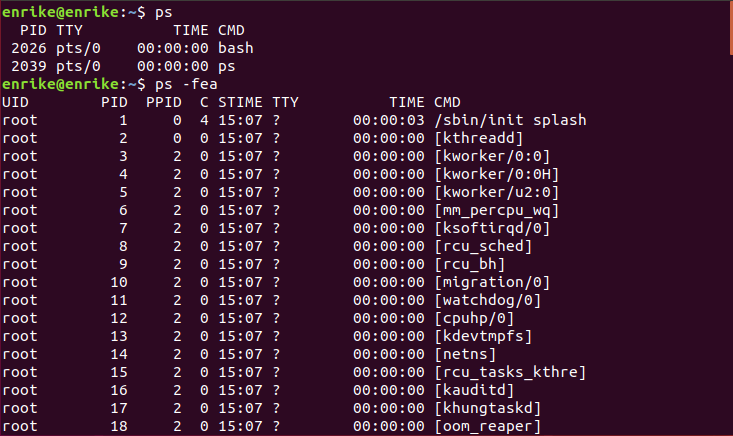
\includegraphics[width=0.85\textwidth]{Practica4/Images/Linux/ps.png}
            \end{figure}
                                      
                                                        
        \end{itemize}
        % PUNTO 2 - A través de la ayuda en linea que proporciona Linux, investigue para que se utiliza el comando ps y mencione las opciones que se pueden utilizar con dicho comando. Además investigue el uso de las llamadas al sistema fork(), execv(), getpid(), getppid() y wait() en la ayuda en líena, mencione que otras funciones similares a execv() existen, reporte sus observaciones
    \newpage     
        \item[\Checkmark] Investigación de las siguientes llamadas al sistema
        \begin{itemize}
        \item \textbf{ps:} “process status”, permite visualizar el estado de un proceso.
Al comando ps se le pueden agregar modificadores como los siguientes:
\begin{itemize}
\item A: Muestra todos los procesos (de todos los usuarios en el sistema).
\item a: Muestra todos los procesos de una consola determinada.
\item d: Muestra todo excepto los líderes de la sesión.
\item e: Muestra todos los procesos (equivalente a -A).
\item T: Muestra todos los procesos de la terminal actual.
\item a: Muestra todos los procesos de la terminal actual incluyendo los de otros usuarios.
\item r: Muestra solamente los procesos corriendo.
\item x: Muestra los procesos en un estilo BSD (sin controlar la terminal).
\end{itemize}


        \item \textbf{fork():} Crea un proceso hijo duplicando la llamada del proceso, este nuevo proceso está referenciado como hijo mientras que el proceso que lo llamó está referenciado como proceso padre.

        \item \textbf{execv():} Crea o reemplaza la imagen de proceso con una nueva imagen de procesos, esta función provee de un arreglo de punteros a cadenas con terminación null la cual representa la lista de argumentos disponibles para la ejecución de un archivo.

        \item \textbf{getpid():} Obtiene el identificador del proceso que lo ejecuta.

        \item \textbf{getppid():} Obtiene el identificador del padre del proceso que lo ejecuta.

        \item \textbf{wait():} Espera o hace esperar al proceso hasta que su estado y /o funciones terminen.   
        
        \item \textbf{Similares a execv():  } exec(), execvpe(), execvp(), execl, execlp, execle.       
        
                                                                        
        \end{itemize}
        
        \item[\Checkmark] \textbf{Punto 3:} Creación de procesos por copia exacta de código
        \begin{multicols}{2}
            \begin{itemize}
                \item Primer código 
                    \inputminted{c++}{Code/Linux/3.c}
                \columnbreak                    
                \item Segundo código
                    \inputminted{c++}{Code/Linux/3_1.c} 
            \end{itemize}
            \end{multicols}
        \newpage            
        \item[\Checkmark] \textbf{Punto 6:} Creación de procesos por sustitución de código
        \begin{multicols}{2}
            \begin{itemize}
                \item Codigo de sustitución
                    \inputminted{c++}{Code/Linux/6.c}
                    \columnbreak                            
                \item Código a ejecutar
                        \inputminted{c++}{Code/Linux/hola.c} 
            \end{itemize}
            \end{multicols}
        \end{itemize}
        
            % ///////////////////////////////////////////////////////////////////////////////////////////////
            %                              SECCIÓN WINDOWS
            % ///////////////////////////////////////////////////////////////////////////////////////////////
    
            \subsubsection{Sección Windows:}
                \begin{itemize}
                    \item[\Checkmark] \textbf{Punto 3:} Creación de un nuevo proceso
                    
                    %PONER CODIGO 3 DE EJEMPLO AQUI

                    \inputminted{c++}{Code/Windows/3.c} 
                    
                    \item[\Checkmark] \textbf{Punto 4:} Programa que contendrá al proceso hijo
                    
                    %PONER CODIGO 4 DE EJEMPLO AQUI
                    \inputminted{c++}{Code/Windows/4.c} 

            
                    \item[\Checkmark] \textbf{Punto 6:} Diferencias y similitudes de creación de procesos en Linux y Windows.

                    Al igual que en Windows, en el sistema operativo Unix existe la creación de procesos por sustitución de código, ambos sistemas operativos al utilizar la creación de procesos por sustitución son muy parecidos, al recibir los argumentos en el main y la forma en la que trabaja.
                    
                    Por otra parte las diferencias encontradas son en la parte de la creación de los procesos, que por obvias razones no puede ser igual debido a las diferencias entre estos dos sistemas operativos. Para el sistema operativo Unix se utilizó la llamada al sistema fork() a diferencia de Windows donde se utilizó la llamada al sistema CreateProcess().

                    \item[\Checkmark] \textbf{Punto 7:} Función \textbf{GetCurrentProcessId()}
                   % AQUI PONER INVESTIGACIÓN
                   
                   GetCurrentProcessId devuelve el identificador de proceso del proceso de llamada.

                    SINTAXIS\\
                    DWORD GetCurrentProcessId (VOID);
                    
                    
                    VALOR DEVUELTO\\
                    El identificador de proceso del proceso de llamada.
                    
                    OBSERVACIONES\\
                    Hasta que el proceso finaliza, el identificador del proceso identifica de manera única el proceso en todo el sistema.
                    
                    RTSSrun devuelve el valor del ID de proceso actual.
                \end{itemize}
        
        % ////////////////////////////////////////////////////////////////////////////////////////////////////
        %                       CODIGOS FUENTE DE LOS PROGRAMAS DESARROLLADOS
        % ////////////////////////////////////////////////////////////////////////////////////////////////////
\newpage

        \subsection{Códigos fuente de los programas desarrollados}
        % AQUI SOLO VA EL CODIGO FUENTE, MÁS ABAJO EXPLICAN LO QUE QUIERAN EN LA PARTE DE EJECUCIÓN :)
        \subsubsection{Sección Linux}

            \begin{itemize}

         \item[\Checkmark] \textbf{Punto 4:} Árbol de procesos del pizarrón por copia exacta de código.
                    \inputminted{c++}{Code/Linux/4.c}
                
                \item[\Checkmark] \textbf{Punto 5:} Operaciones con matrices de 10x10 con creación de seis procesos por copia exacta de código y de forma secuencial. Medición de ambos tiempos.

                    \begin{itemize}
                        \item \textbf{Aplicación secuencial}
                            \inputminted{c++}{Code/Linux/operacionesMatrices.c}
                            
                        \item \textbf{Aplicación con seis procesos por copia exacta de código}
                            \inputminted{c++}{Code/Linux/5.c}  
                        
                        \item \textbf{Código para el tiempo}
                            \inputminted{c++}{Code/Linux/tiempo.h}  
                        
                        \item \textbf{Código objeto para el tiempo}
                            \inputminted{c++}{Code/Linux/tiempo.c}  
                            
                    \end{itemize}
                
                \item[\Checkmark] \textbf{Punto 7:} Creación de tres procesos por sustitución de código que ejecutarán: Expresión aritmética, cambio de permisos a archivos e inversas de dos matrices.

                    \begin{itemize}
                        \item \textbf{Aplicación con tres procesos por sustitución de código}
                            \inputminted{c++}{Code/Linux/7.c}
                        
                        \item \textbf{Expresión aritmética}
                            \inputminted{c++}{Code/Linux/expresion.c}
                        \newpage
                        \item \textbf{Permisos de archivos}
                            \inputminted{c++}{Code/Linux/permisos.c}

                        \item \textbf{Inversas de matrices}
                            \inputminted{c++}{Code/Linux/7_inversa.c} 
                            
                    \end{itemize}
                \newpage
                \item[\Checkmark] \textbf{Punto 8:} Operaciones con matrices de 10x10 con creación de seis procesos por sustitución código.
                    

                    \begin{itemize}
                        \item \textbf{Aplicación con seis procesos por sustitución de código}
                            \inputminted{c++}{Code/Linux/8.c}
                            
                        \item \textbf{Suma de matrices}
                            \inputminted{c++}{Code/Linux/suma.c}

                        \item \textbf{Resta de matrices}
                            \inputminted{c++}{Code/Linux/resta.c}

                        \item \textbf{Multiplicación de matrices}
                            \inputminted{c++}{Code/Linux/multiplicacion.c}  

                        \item \textbf{Transpuestas de matrices}
                            \inputminted{c++}{Code/Linux/transpuesta.c}

                        \item \textbf{Inversas de matrices}
                            \inputminted{c++}{Code/Linux/inversa.c}
                            
                        \item \textbf{Leer archivos con resultados}
                            \inputminted{c++}{Code/Linux/leerArchivos.c}

                        % Poner los que sean necesarios
                    \end{itemize}
       \end{itemize}
\item 
        
        \subsubsection{Sección Windows}
        
        \begin{itemize}

            \item[\Checkmark] \textbf{Punto 5:} Programa que contendrá al proceso hijo, con un nuevo argumento.
                \begin{itemize}
                    \item Proceso padre
                    \inputminted{c++}{Code/Windows/5.c}
                    
                    \item Proceso hijo
                    \inputminted{c++}{Code/Windows/5_hijo.c}
                \end{itemize}
                

            \item[\Checkmark] \textbf{Punto 7:} Árbol de procesos que imprimen su identificador.
                \begin{itemize}
                    \item Main
                    \inputminted{c++}{Code/Windows/7.c}
                    
                    \item Un proceso hijo-padre
                    \inputminted{c++}{Code/Windows/7_padre.c}
                    
                    \item Cinco procesos hijos
                    \inputminted{c++}{Code/Windows/7_hijo.c}
                    
                    \item Tres procesos nietos por cada hijo
                    \inputminted{c++}{Code/Windows/7_nieto.c}
                \end{itemize}

            \item[\Checkmark] \textbf{Punto 8:} Operaciones con matrices de 10x10 con creación de seis procesos por copia exacta de código y de forma secuencial. Medición de ambos tiempos.

                \begin{itemize}
                    \item \textbf{Aplicación secuencial}
                            \inputminted{c++}{Code/Windows/8_1.c}
                            
                        \item \textbf{Aplicación con seis procesos}
                        \begin{itemize}
                        \item \textbf{Main}
                            \inputminted{c++}{Code/Windows/8.c}
                            \newpage
                        \item \textbf{Suma de matrices}
                            \inputminted{c++}{Code/Windows/suma.c}

                        \item \textbf{Resta de matrices}
                            \inputminted{c++}{Code/Windows/resta.c}

                        \item \textbf{Multiplicación de matrices}
                            \inputminted{c++}{Code/Windows/multiplicacion.c}  

                        \item \textbf{Transpuestas de matrices}
                            \inputminted{c++}{Code/Windows/transpuesta.c}

                        \item \textbf{Inversas de matrices}
                            \inputminted{c++}{Code/Windows/inversa.c}
                            
                        \item \textbf{Leer archivos con resultados}
                            \inputminted{c++}{Code/Windows/leerArchivos.c}

                        % Poner los que sean necesarios
                    \end{itemize}
                              
                \end{itemize}
            
        \end{itemize}
        
        % ////////////////////////////////////////////////////////////////////////////////////////////////////
        %                               PANTALLAS DE EJECUCIÓN DE LOS PROGRAMAS DESARROLLADOS
        % ////////////////////////////////////////////////////////////////////////////////////////////////////
        
        \newpage
        \subsection{Pantallas de ejecución de los programas desarrollados}

            % ///////////////////////////////////////////////////////////////////////////////////////////////
            %                                           SECCION LINUX
            % ///////////////////////////////////////////////////////////////////////////////////////////////
                        
            % AQUI SI VAN LAS EXPLICACIONES QUE SEAN NECESARIAS         
            \subsubsection{Sección Linux:}
            \begin{itemize}
                \item[\Checkmark] \textbf{Punto 3:} Creación de procesos por copia exacta de código
                
                    \begin{itemize}
                        \item \textbf{Primer código}
                           \begin{figure}[h!]
                                \centering
                                 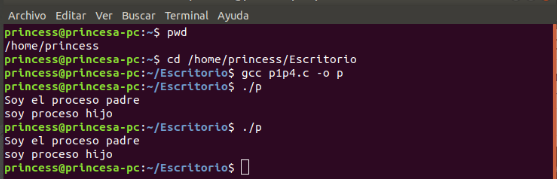
\includegraphics[width=0.9\textwidth]{Practica4/Images/Linux/3_1.png}
                                \caption{Ejecución del primer código}
                            \end{figure}  
                                                  \item \textbf{Segundo código}
                                                  
                            En el funcionamiento del segundo código, en esta caso, pasa el primer proceso e imprime el ultimo mensaje,  posteriormente el siguiente proceso, e igualmente imprime el mensaje,  y termina el programa.
                            \begin{figure}[h!]
                                \centering
                                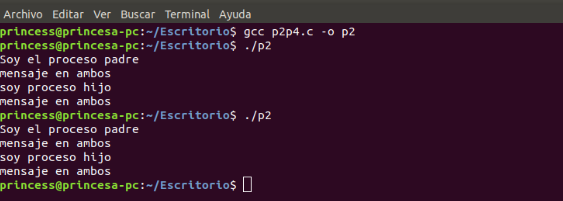
\includegraphics[width=0.9\textwidth]{Practica4/Images/Linux/3_2.png}
                                \caption{Ejecución del segundo código}
                            \end{figure}

                
             \end{itemize}
                \newpage
                \item[\Checkmark] \textbf{Punto 4:} Árbol de procesos del pizarrón por copia exacta de código.

        
                \begin{figure}[h!]
                  \centering
                    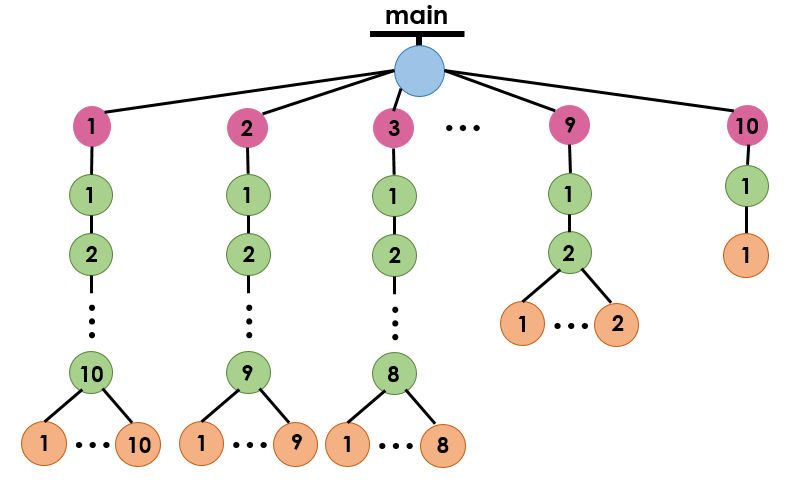
\includegraphics[width=0.8\textwidth]{Practica4/Images/Linux/arbol4.PNG}                        \caption{Árbol mostrado en el pizarrón}
                \end{figure}
                
                \begin{figure}[h!]
                  \centering
                    \includegraphics[width=0.8\textwidth]{Practica4/Images/Linux/arbolp4.png} 
                    \caption{Árbol de procesos con su identificador}
                \end{figure}
               \newpage
                \begin{figure}[h!]
                \centering
                    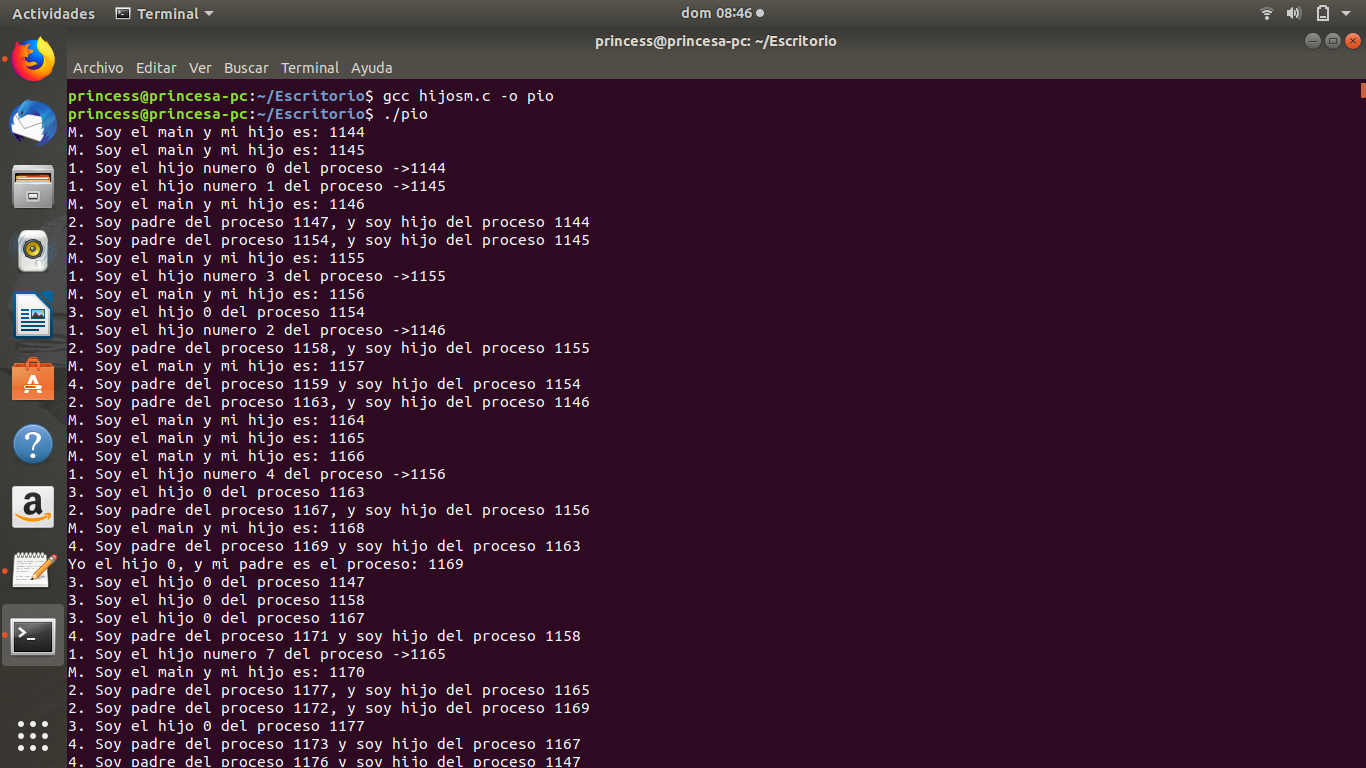
\includegraphics[width=\textwidth]{Practica4/Images/Linux/4_1.png}
                    \caption{Ejecución del punto 4}
                     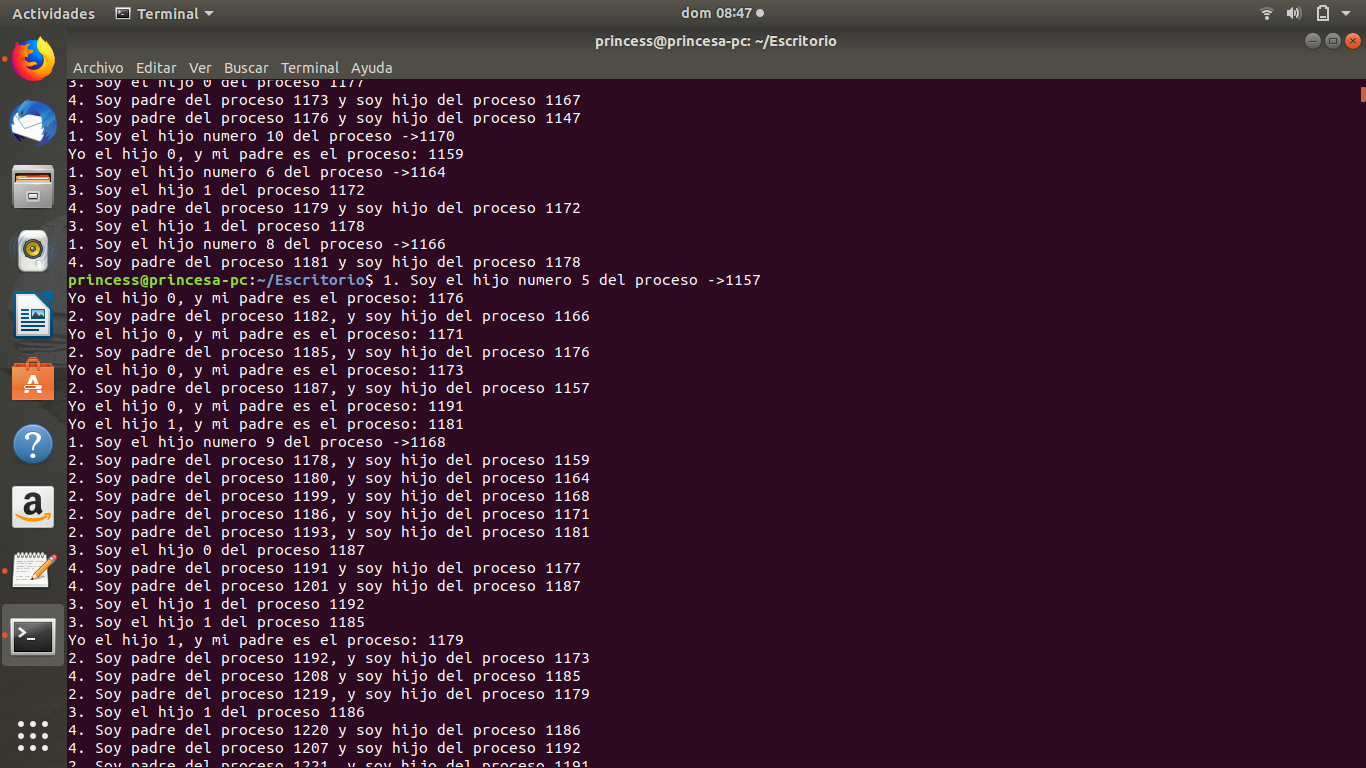
\includegraphics[width=\textwidth]{Practica4/Images/Linux/4_2.png}
                    \caption{Ejecución del punto 4}
                \end{figure}
\newpage
                \begin{figure}[h!]
                \centering
                    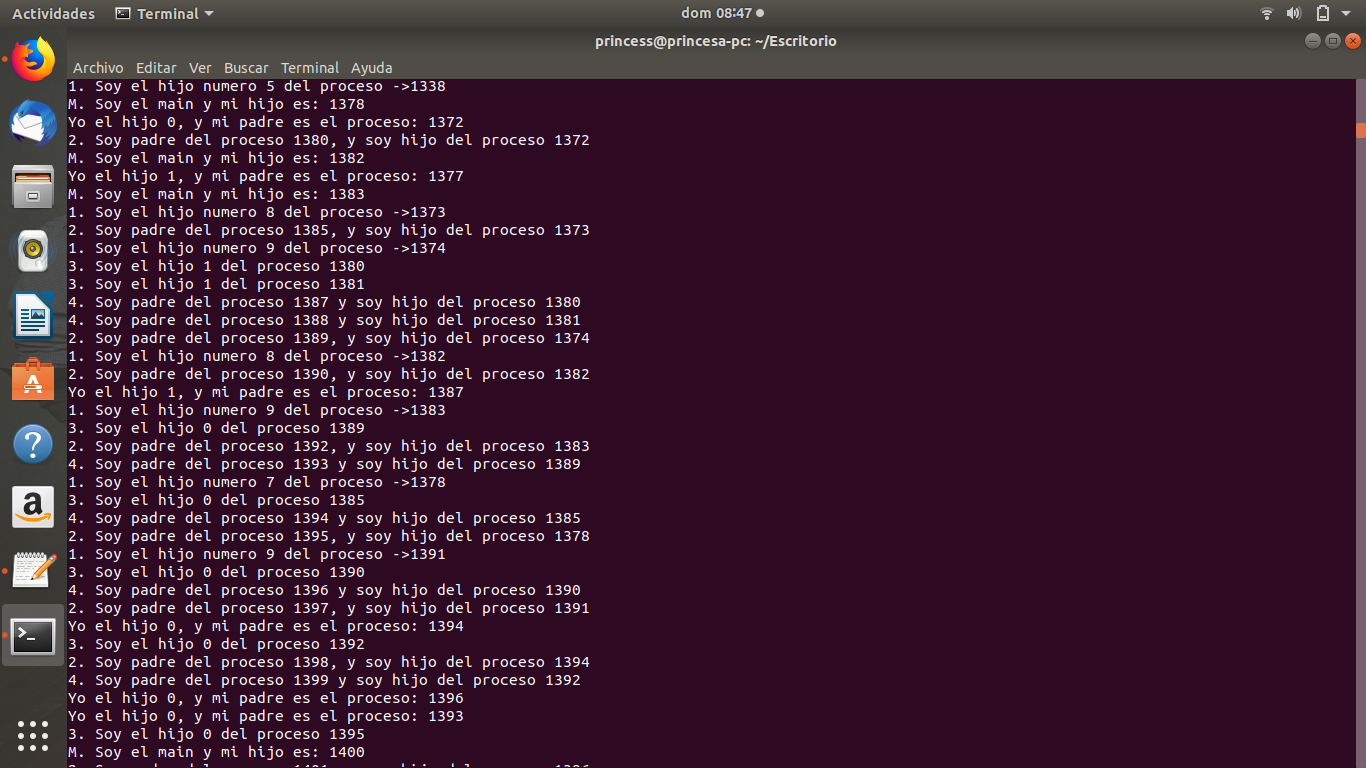
\includegraphics[width=\textwidth]{Practica4/Images/Linux/4_3.png}
                    \caption{Ejecución del punto 4}

                    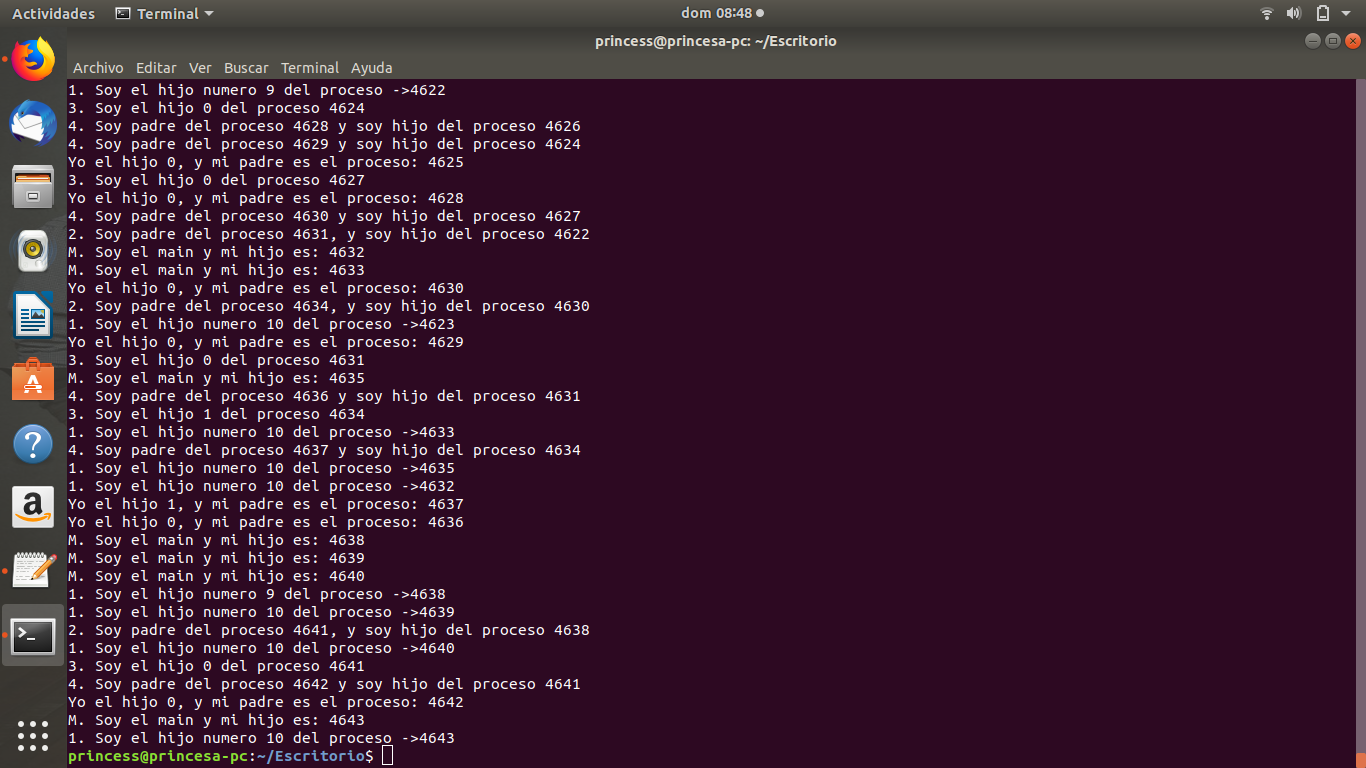
\includegraphics[width=\textwidth]{Practica4/Images/Linux/4_4.png}
                    \caption{Ejecución del punto 4}
                \end{figure}
                   
                

                    % AQUI PUEDES PONER COMENTARIOS QUE SEAN NECESARIOS
            Se crean los procesos con un numero de identificador diferente cada vez que se ejecuta el programa. El administrador de procesos es quien va marcando la prioridad para el orden de la construcción de los procesos.
                
                \newpage
                \item[\Checkmark] \textbf{Punto 5:} Operaciones con matrices de 10x10 con creación de seis procesos por copia exacta de código y de forma secuencial. Medición de ambos tiempos.
                    
                    \begin{figure}[h!]
                        \centering
                        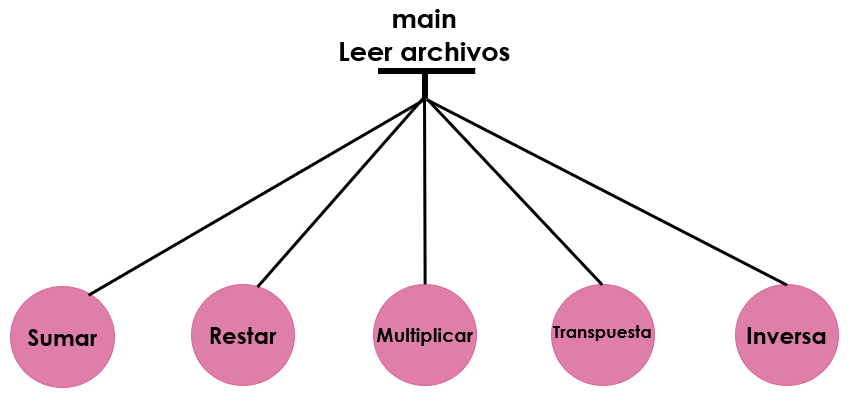
\includegraphics[width=0.8\textwidth]{Practica4/Images/arbol5.PNG}
                        \caption{Árbol de los procesos punto 5}
                    \end{figure}

                    \begin{itemize}
                        \item \textbf{Aplicación secuencial}
                            \begin{figure}[h!]
                                \centering
                                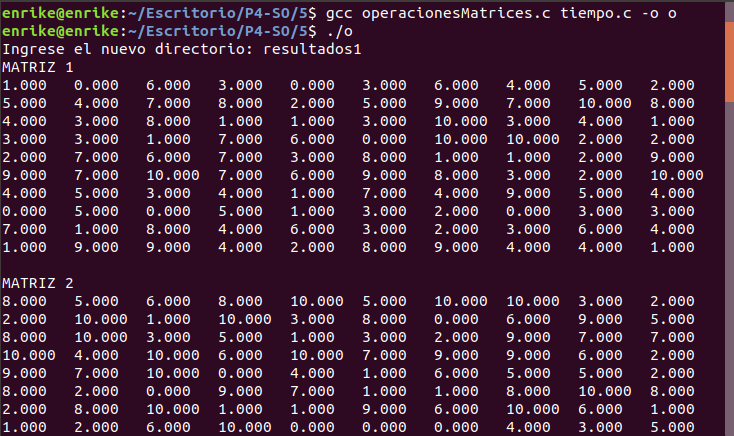
\includegraphics[width=0.8\textwidth]{Practica4/Images/Linux/5_1.png}
                                \caption{Genera matrices aleatorias}
                                
                                
                               \end{figure}
                               \newpage
                               \begin{figure}[h!]
                                \centering
                               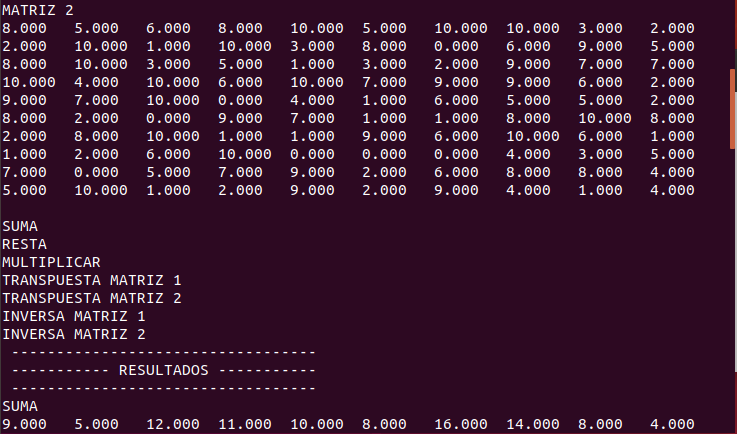
\includegraphics[width=0.67\textwidth]{Practica4/Images/Linux/5_2.png}
                                \caption{Realiza operaciones de matrices de forma secuencial y genera archivos de resultados}
                                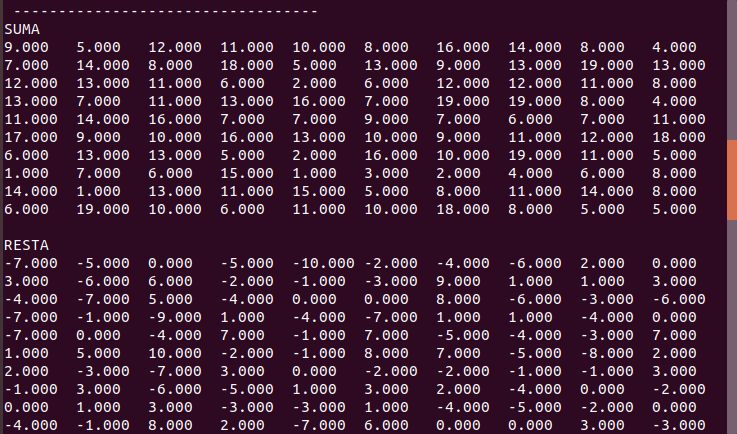
\includegraphics[width=0.67\textwidth]{Practica4/Images/Linux/5_3.png}
                                \caption{Lee resultados de suma y resta}
                                
                                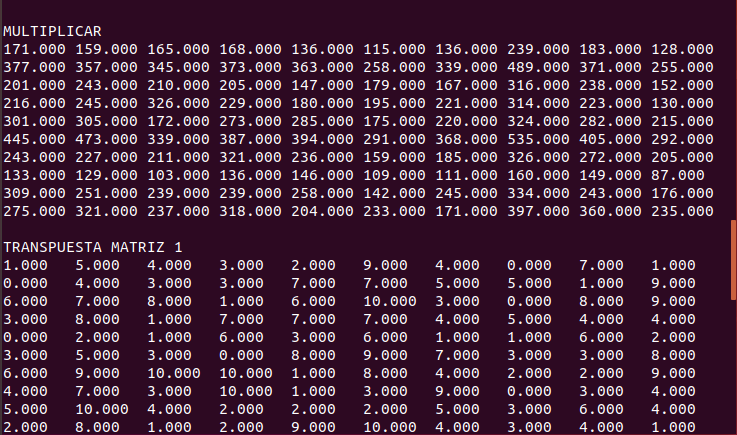
\includegraphics[width=0.67\textwidth]{Practica4/Images/Linux/5_4.png}
                                \caption{Lee resultados de multiplicación y transpuestas}
                                
                            \end{figure}
                            \newpage
                            \begin{figure}[h!]
                                \centering
                                
                                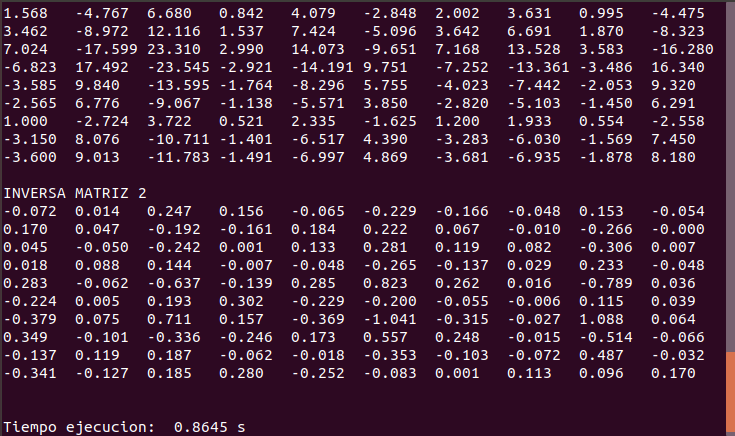
\includegraphics[width=0.75\textwidth]{Practica4/Images/Linux/5_5.png}
                                \caption{Lee resultados de inversas y muestra el tiempo de ejecución.}
                                 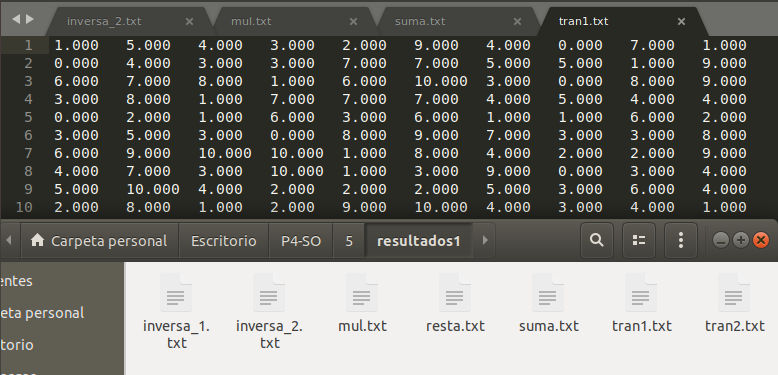
\includegraphics[width=0.75\textwidth]{Practica4/Images/Linux/5_6.png}
                                \caption{Archivos de resultados generados}
                            \end{figure}

                            % AQUI PUEDES PONER COMENTARIOS QUE SEAN NECESARIOS

                        \newpage
                        \item \textbf{Aplicación con seis procesos por copia exacta de código}
                            \begin{figure}[h!]
                                \centering
                                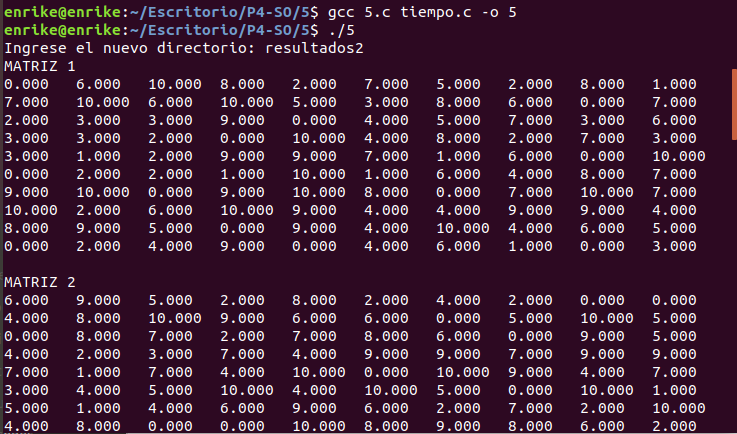
\includegraphics[width=0.67\textwidth]{Practica4/Images/Linux/5_7.png}
                                \caption{Genera matrices aleatorias}
                                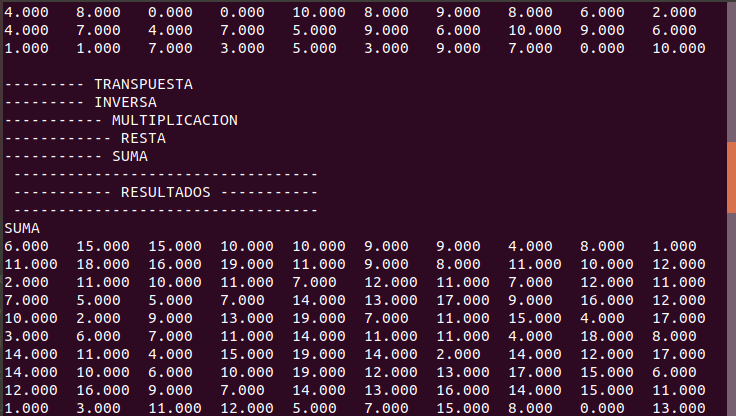
\includegraphics[width=0.67\textwidth]{Practica4/Images/Linux/5_8.png}
                                \caption{Operaciones con procesos y genera archivos de resultados. Lee resultados de suma}
                                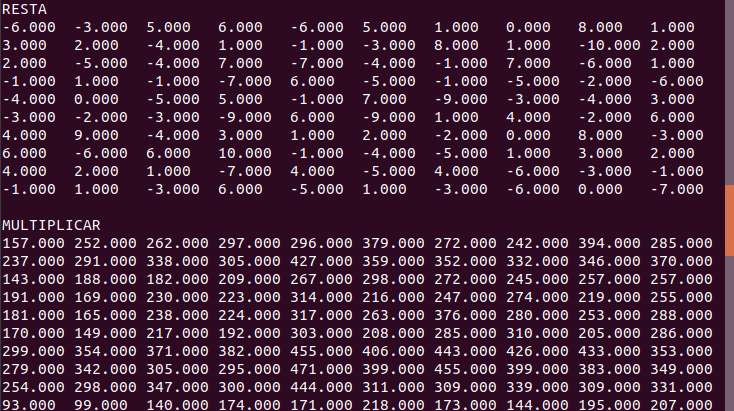
\includegraphics[width=0.67\textwidth]{Practica4/Images/Linux/5_9.png}
                                \caption{Lee resultados de resta y multiplicación}
                            \end{figure}
                            \newpage
                            \begin{figure}[h!]
                                \centering
                                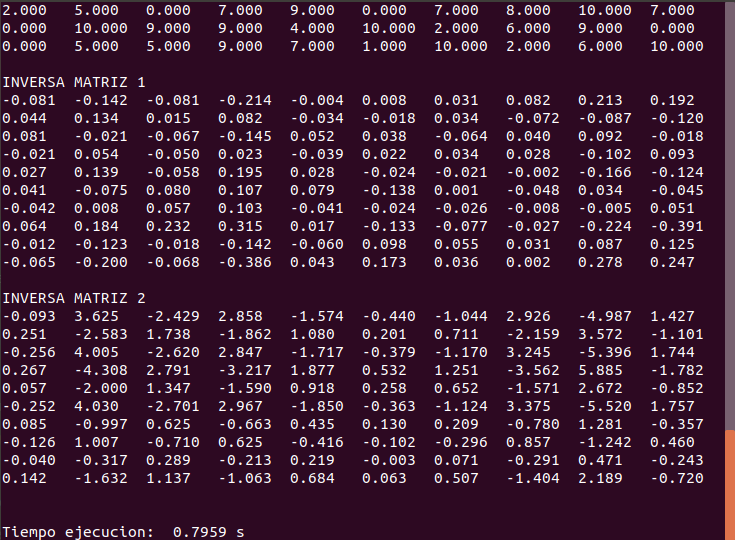
\includegraphics[width=0.73\textwidth]{Practica4/Images/Linux/5_10.png}
                                \caption{Lee resultados de inversas y muestra el tiempo de ejecución.}
                                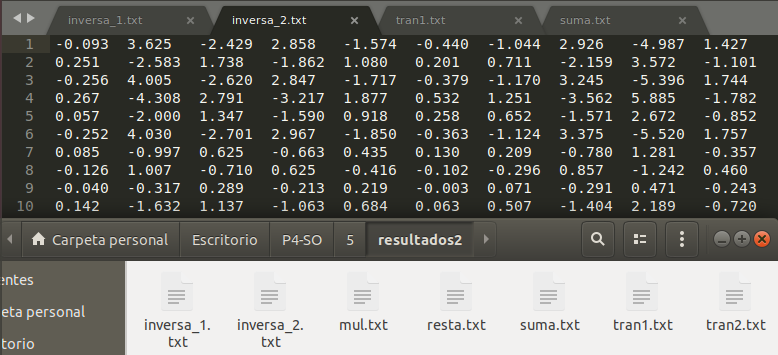
\includegraphics[width=0.73\textwidth]{Practica4/Images/Linux/5_11.png}
                                \caption{Archivos de resultados generados}
                            \end{figure}

                            % AQUI PUEDES PONER COMENTARIOS QUE SEAN NECESARIOS
                          
                    \end{itemize}
                    

                \item[\Checkmark] \textbf{Punto 6:} Creación de procesos por copia exacta de código
                
                \begin{figure}[h!]
                    \centering
                    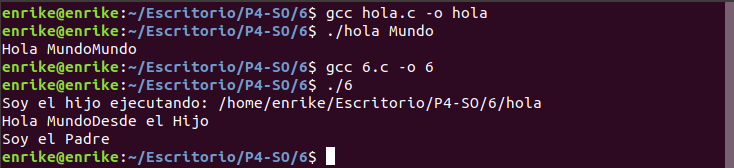
\includegraphics[width=0.78\textwidth]{Practica4/Images/Linux/6.png}
                    \caption{El programa que posee al proceso padre (en este caso el main del código) recibe como argumento la ruta del ejecutable del código que contendrá al proceso hijo (en este caso un ''Hola Mundo'').}
                \end{figure}

                \newpage
                \item[\Checkmark] \textbf{Punto 7:} Creación de tres procesos por sustitución de código que ejecutarán: Expresión aritmética, cambio de permisos a archivos e inversas de dos matrices.
                    \begin{figure}[h!]
                        \centering
                         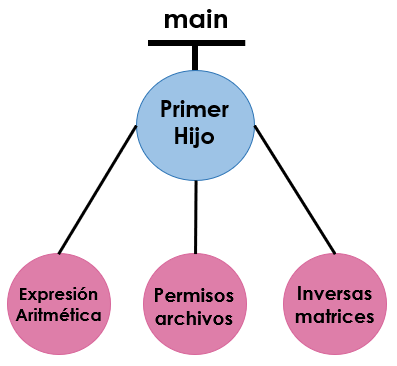
\includegraphics[width=0.39\textwidth]{Practica4/Images/Linux/arbol7.PNG}
                        \caption{Árbol de los procesos punto 7}
                         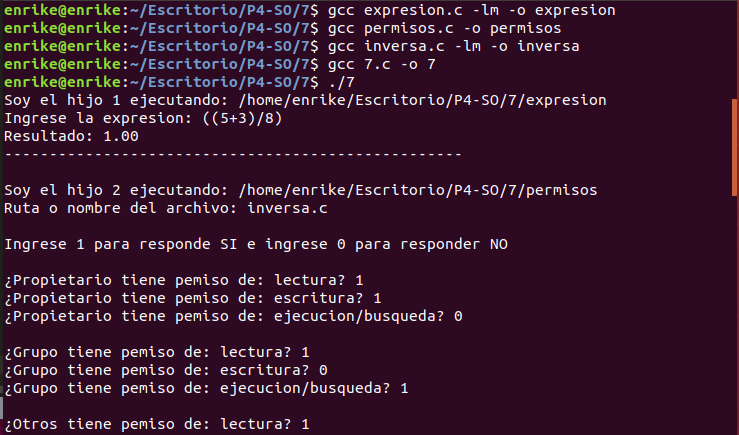
\includegraphics[width=0.65\textwidth]{Practica4/Images/Linux/7_1.png}
                        \caption{Proceso de expresión aritmética y cambio de permisos a archivos}
                        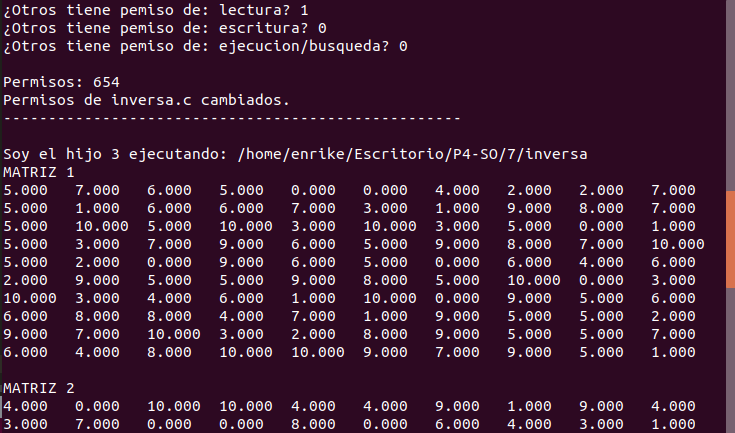
\includegraphics[width=0.65\textwidth]{Practica4/Images/Linux/7_2.png}
                        \caption{Genera dos matrices aleatorias}
                        
                \end{figure}

                \newpage
                   \begin{figure}[h!]
                        \centering
                        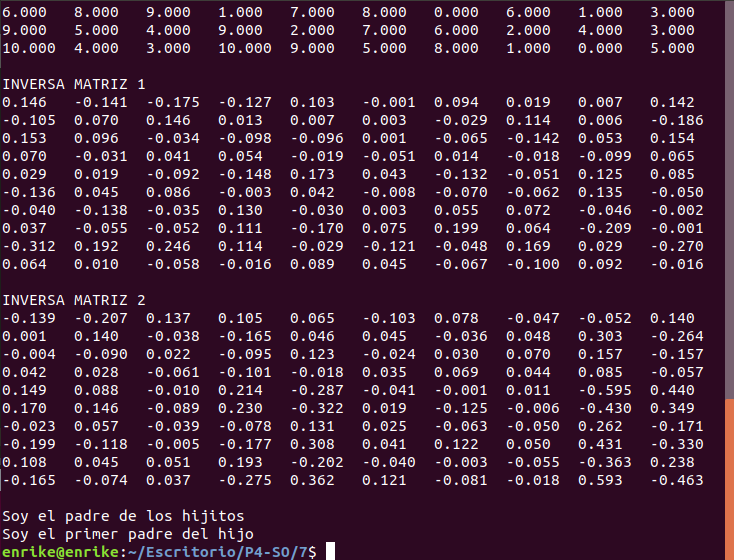
\includegraphics[width=0.85\textwidth]{Practica4/Images/Linux/7_3.png}
                        \caption{Proceso de inversas de matrices}

                    \end{figure}

                   \begin{figure}[h!]
                        \centering 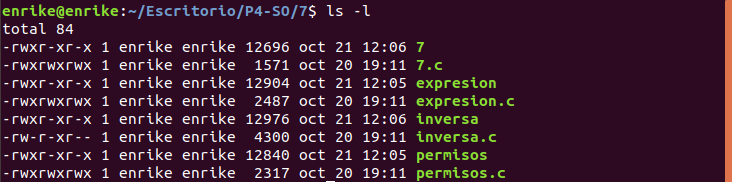
\includegraphics[width=0.85\textwidth]{Practica4/Images/Linux/7_5.png}
                        \caption{Verificación del cambio de permisos en el archivo ''inversa.c''}
                    \end{figure}

                    Un funcionamiento 100\% concurrente es imposible en aplicaciones que utilizan creación de códigos por sustitución de código y por copia exacta de código.
                
                Por ejemplo, en esta aplicación, se requiere que se ingrese por medio del teclado muchas entradas, que se manejarán como variables dentro de la ejecución de cada proceso. 
                
                Si intentáramos que la aplicación sea concurrente, las entradas exclusivas y correspondientes a cada proceso se mezclarían y los procesos no sabrían identificar cual es su entrada correcta, por lo que arrojarían múltiples errores.
                
                Para evitar esto, colocamos la llamada al sistema \textbf{wait()} por cada proceso que este realizando nuestra aplicación, para darle tiempo al usuario de que ingrese la entrada correcta, así como al mismo proceso para que realice las operaciones que tenga que realizar, y no existan colisiones entre las variables de éstos.
                    % AQUÍ PUEDES PONER COMENTARIOS QUE SEAN NECESARIOS
                \newpage                
                \item[\Checkmark] \textbf{Punto 8:} Operaciones con matrices de 10x10 con creación de seis procesos por sustitución código.
                \begin{figure}[h!]
                        \centering
                        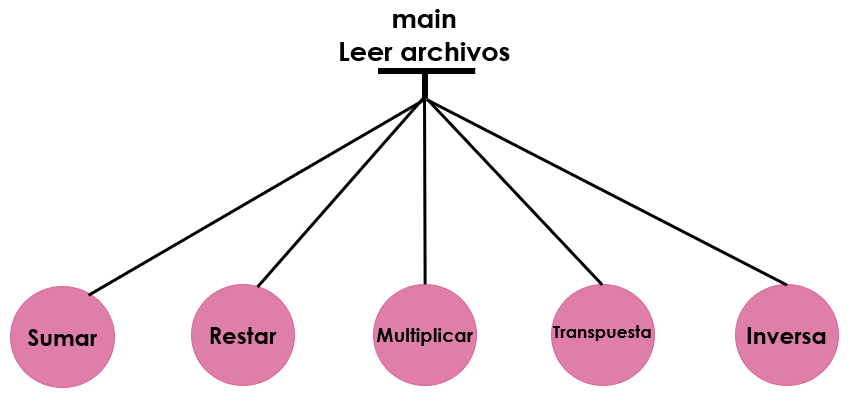
\includegraphics[width=0.88\textwidth]{Practica4/Images/arbol5.PNG}
                        \caption{Árbol de los procesos punto 8. Es el mismo que el del punto 5}
                        
                        \end{figure}

                    \begin{figure}[h!]
                        \centering
                        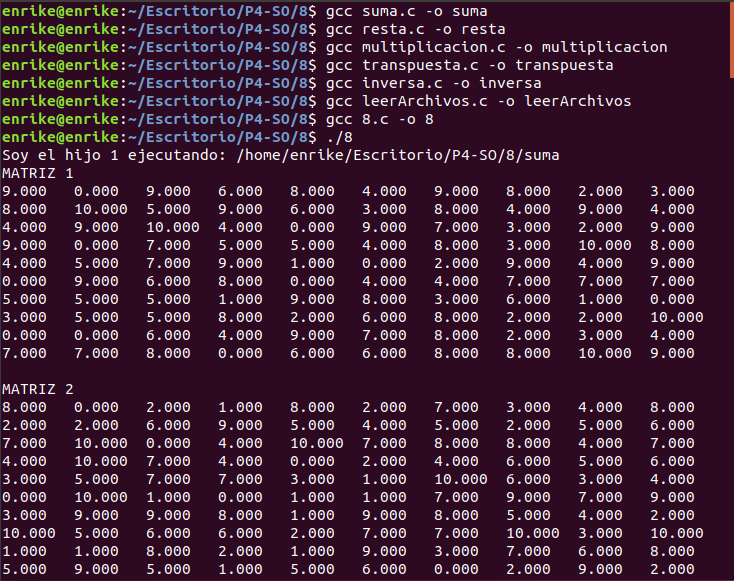
\includegraphics[width=0.88\textwidth]{Practica4/Images/Linux/8_1.png}
                        \caption{Proceso Hijo 1: Ejecuta la suma y genera archivo de resultados}
                    \end{figure}
                \newpage
                    \begin{figure}[h!]
                        \centering
                        
                        
                        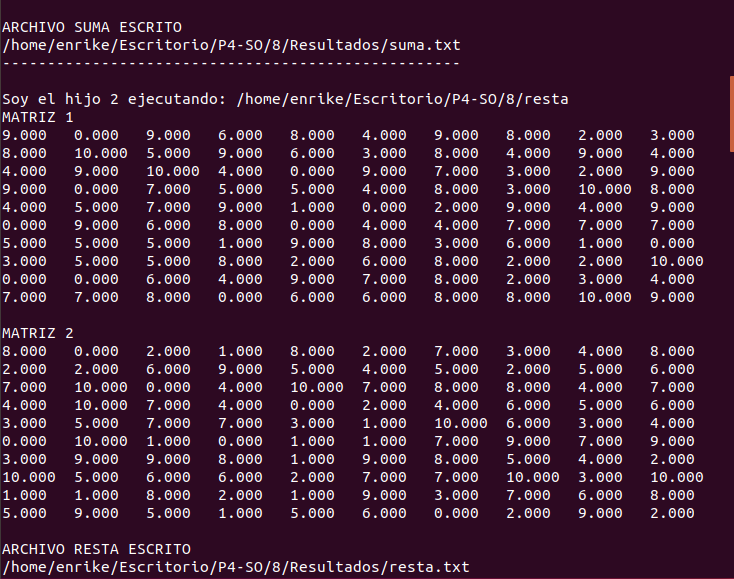
\includegraphics[width=0.82\textwidth]{Practica4/Images/Linux/8_2.png}
                        \caption{Proceso Hijo 2: Ejecuta la resta y genera archivo de resultados}
                        
                        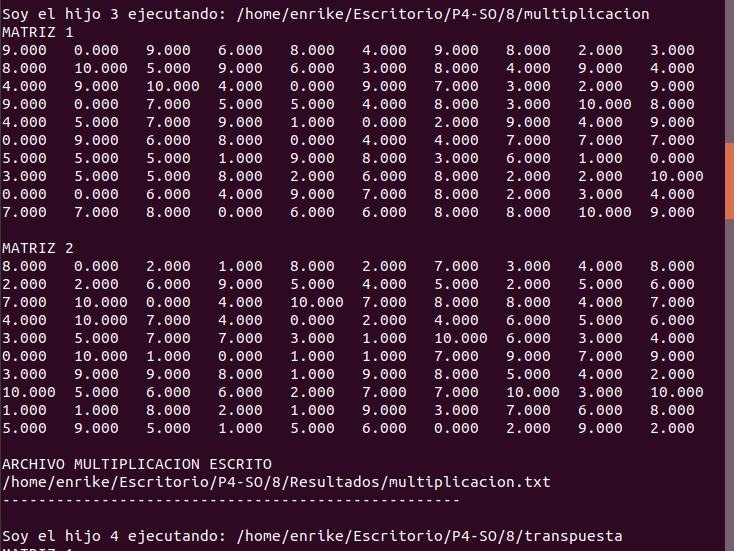
\includegraphics[width=0.82\textwidth]{Practica4/Images/Linux/8_4.png}
                        \caption{Proceso Hijo 3: Ejecuta la multiplicación y genera archivo de resultados}
                        
                    \end{figure}
                    \clearpage
                    \begin{figure}[h!]
                        \centering
                        
                        
                      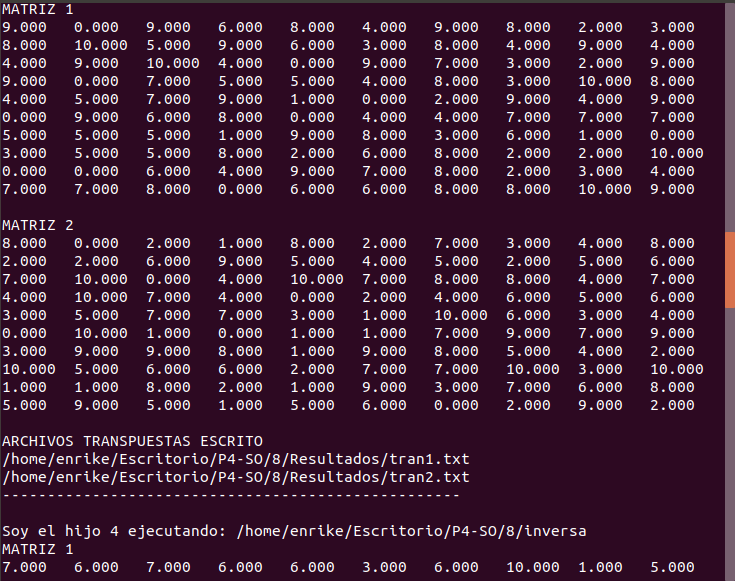
\includegraphics[width=0.82\textwidth]{Practica4/Images/Linux/8_5.png}
                        \caption{Proceso Hijo 4: Ejecuta las transpuestas y genera dos archivos de resultados}
                        
                        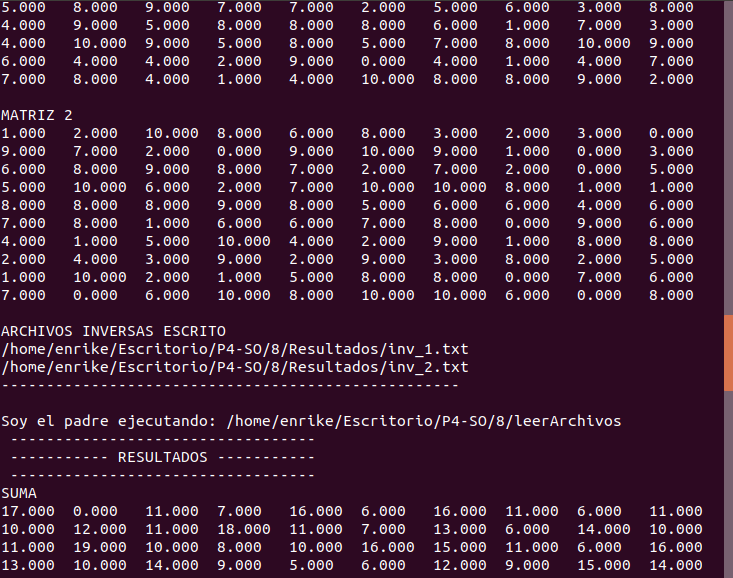
\includegraphics[width=0.82\textwidth]{Practica4/Images/Linux/8_6.png}
                        \caption{Proceso Hijo 5: Ejecuta las inversas y genera dos archivos de resultados}
                        
                    \end{figure}
                    \clearpage
                    \begin{figure}[h!]
                        \centering
                        
                        
                        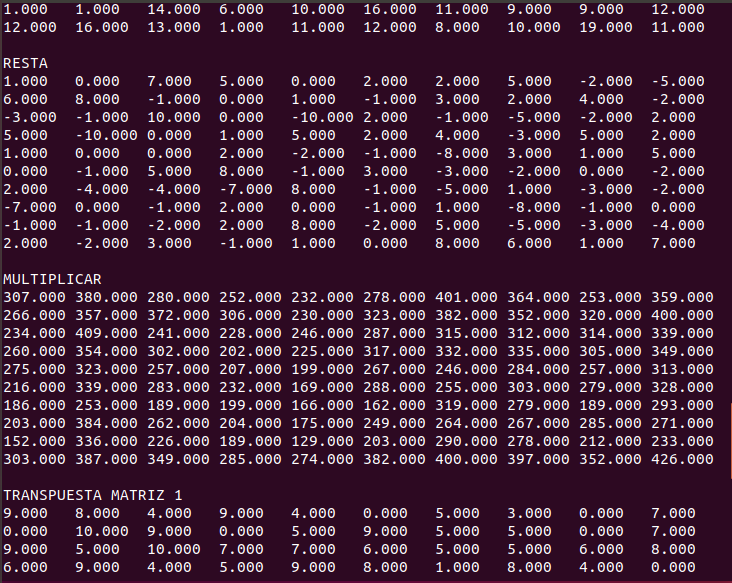
\includegraphics[width=0.82\textwidth]{Practica4/Images/Linux/8_7.png}
                        \caption{Proceso Sub-Padre (6): Lee archivos de resultados y los despliega en la consola}
                        
                        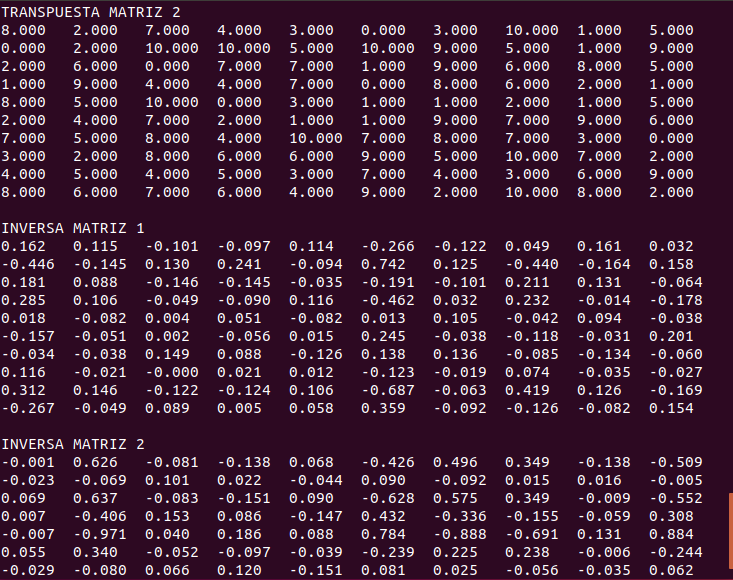
\includegraphics[width=0.82\textwidth]{Practica4/Images/Linux/8_9.png}
                        \caption{Lee archivos de resultados de matrices transpuestas e inversas}
                        
                    \end{figure}
                    \clearpage
                    \begin{figure}[h!]
                        \centering
                        
                        
                        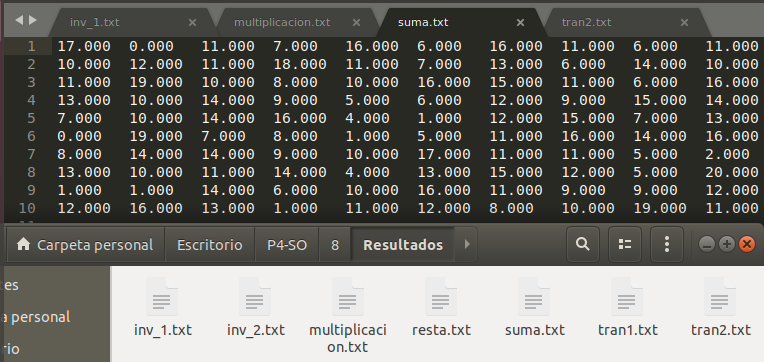
\includegraphics[width=0.95\textwidth]{Practica4/Images/Linux/8_10.png}
                        \caption{Archivos generados durante la ejecución de cada proceso}
                        
                    \end{figure}

                    % AQUÍ PUEDES PONER COMENTARIOS QUE SEAN NECESARIOS
           \end{itemize}

        
             
            % ///////////////////////////////////////////////////////////////////////////////////////////////
            %                                           SECCION WINDOWS
            % ///////////////////////////////////////////////////////////////////////////////////////////////               
   
            \subsubsection{Sección Windows}
        \begin{itemize}
            \item[\Checkmark] \textbf{Punto 3:} Programa de creación de un nuevo proceso.   
                \begin{figure}[h!]
                    \centering
                    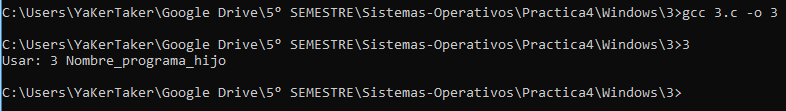
\includegraphics[width=0.95\textwidth]{Practica4/Images/Windows/3.PNG}
                \end{figure}
                % AQUÍ PUEDES PONER COMENTARIOS QUE SEAN NECESARIOS
            
            \item[\Checkmark] \textbf{Punto 4:} Programa que contendrá al proceso hijo.     
                \begin{figure}[h!]
                    \centering
                    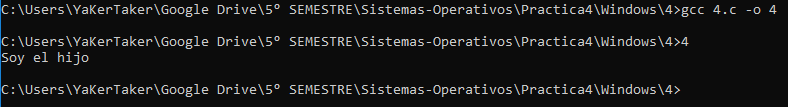
\includegraphics[width=0.95\textwidth]{Practica4/Images/Windows/4.PNG}
                \end{figure}

                % AQUÍ PUEDES PONER COMENTARIOS QUE SEAN NECESARIOS
                
            \item[\Checkmark] \textbf{Punto 5:} Programa que contendrá al proceso hijo, con un nuevo argumento.
                
                \begin{figure}[h!]
                    \centering
                    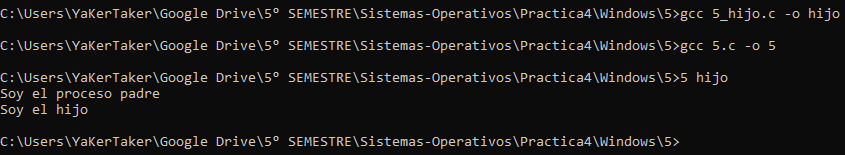
\includegraphics[width=0.95\textwidth]{Practica4/Images/Windows/5.PNG}
                \end{figure}
            \newpage
                % AQUÍ PUEDES PONER COMENTARIOS QUE SEAN NECESARIOS
            \item[\Checkmark] \textbf{Punto 7:} Árbol de procesos que imprimen su identificador.
            
             \begin{figure}[h!]
                    \centering
                    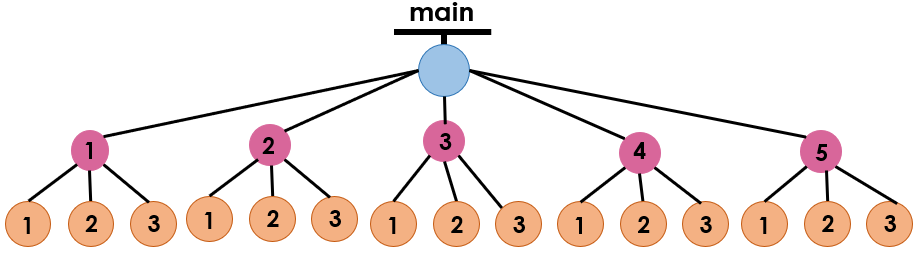
\includegraphics[width=0.8\textwidth]{Practica4/Images/Windows/arbol7.PNG}
                    \caption{Árbol de los procesos punto 7}
            \end{figure}

                \begin{figure}[h!]
                    \centering
                    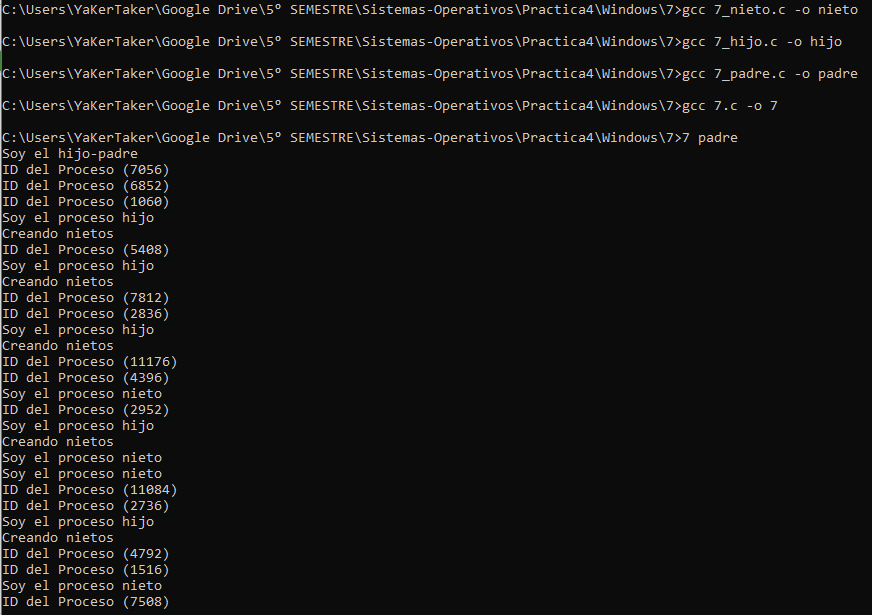
\includegraphics[width=0.9\textwidth]{Practica4/Images/Windows/7_1.PNG}
 
                    
                    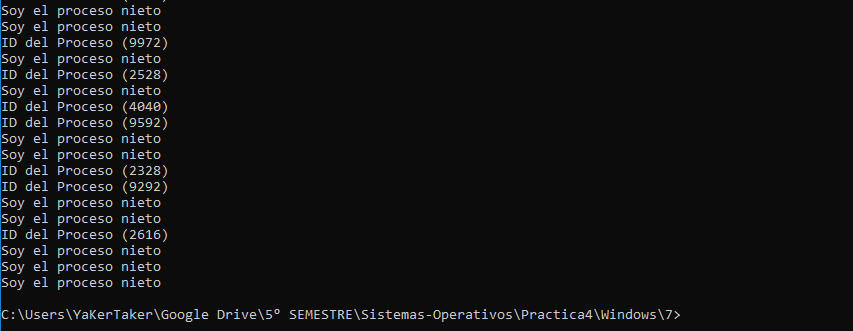
\includegraphics[width=0.9\textwidth]{Practica4/Images/Windows/7_2.PNG}
                \end{figure}

                % AQUÍ PUEDES PONER COMENTARIOS QUE SEAN NECESARIOS
            \newpage
            \item[\Checkmark] \textbf{Punto 8:} Operaciones con matrices de 10x10 con creación de seis procesos por sustitución de código y de forma secuencial. Medición de ambos tiempos.

                \begin{itemize}
                    \item \textbf{Aplicación secuencial}
                    \begin{figure}[h!]
                        \centering
                         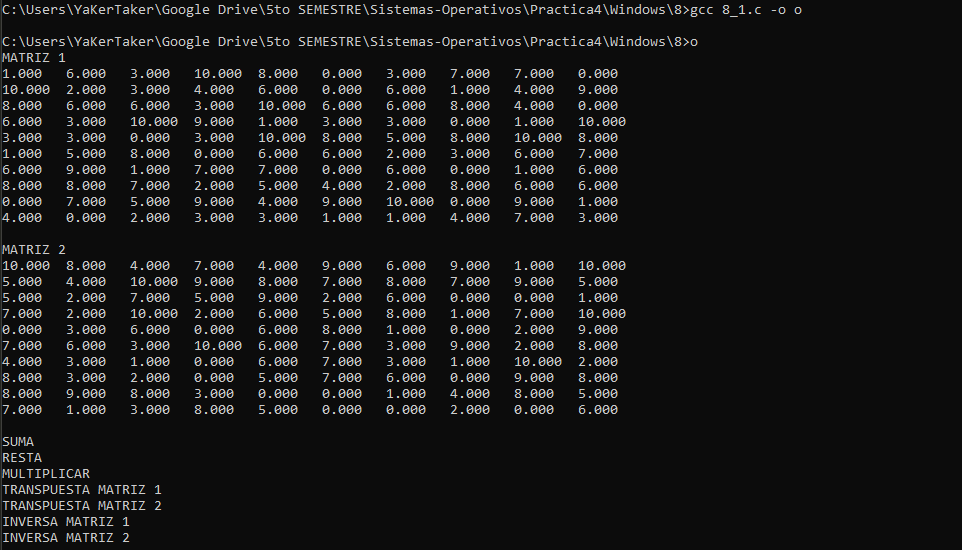
\includegraphics[width=0.9\textwidth]{Practica4/Images/Windows/8_9.PNG}
                        \caption{Genera matrices aleatorias, realiza operaciones de forma secuencial y genera archivos de resultados}
                        
                        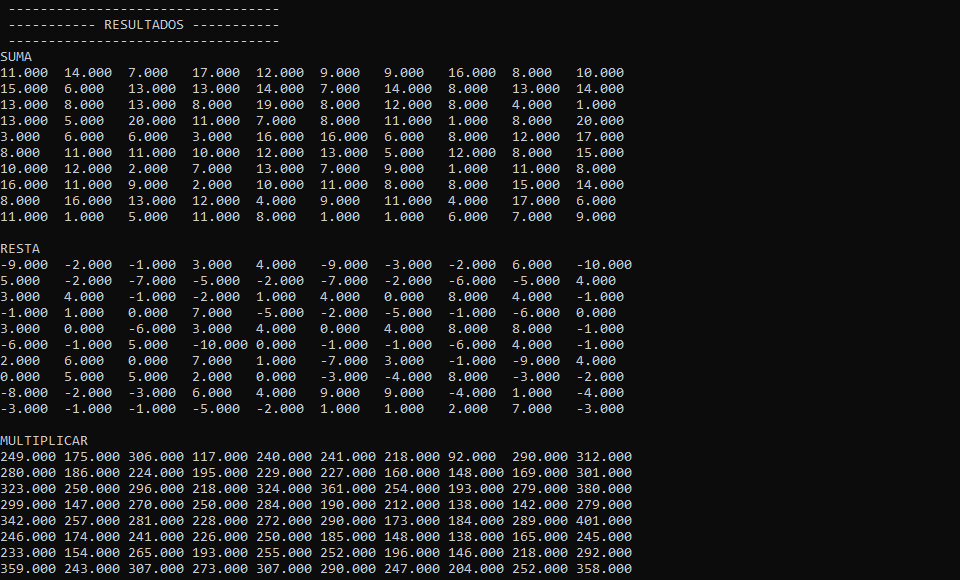
\includegraphics[width=0.9\textwidth]{Practica4/Images/Windows/8_10.PNG}
                        \caption{Lee resultados de suma, resta y multiplicación}
                        
                    \end{figure}
                    
                    \begin{figure}[h!]
                        \centering
                        
                        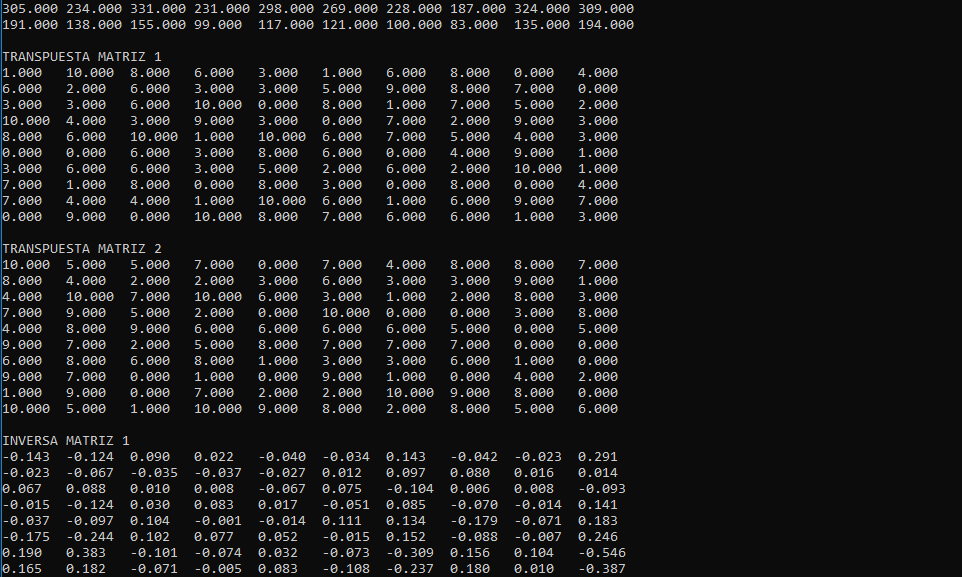
\includegraphics[width=0.9\textwidth]{Practica4/Images/Windows/8_11.PNG}
                        \caption{Lee resultados de matrices transpuestas}
                        
                        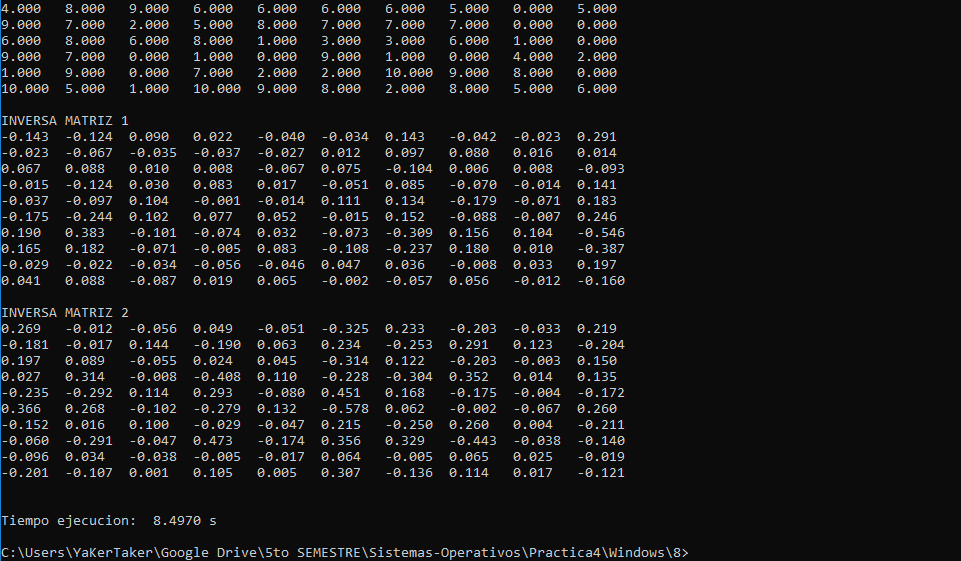
\includegraphics[width=0.9\textwidth]{Practica4/Images/Windows/8_12.PNG}
                        \caption{Lee resultados de matrices inversas. Tiempo de ejecución}
                        
                    \end{figure}
                    \clearpage
                    \begin{figure}[h!]
                        \centering
                        
                        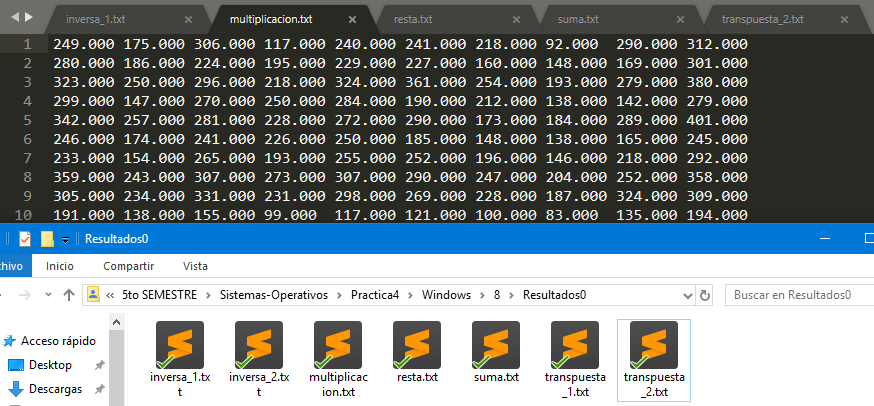
\includegraphics[width=0.9\textwidth]{Practica4/Images/Windows/8_13.PNG}
                        \caption{Archivos  de resultados generados}
                        
                        
                    \end{figure}
                    

                        % AQUI PUEDES PONER COMENTARIOS QUE SEAN NECESARIOS
                    
                    \item \textbf{Aplicación con seis procesos por copia exacta de código}
                         \begin{figure}[h!]
                        \centering
                        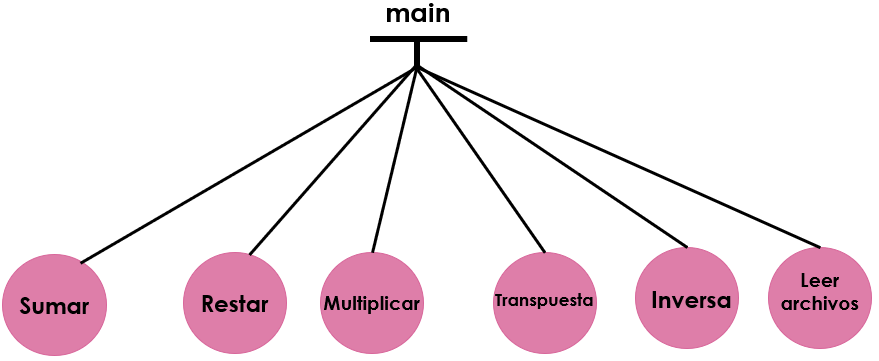
\includegraphics[width=0.75\textwidth]{Practica4/Images/Windows/arbol8.PNG}
                        \caption{Árbol de procesos para el punto 8}
                        \includegraphics[width=0.88\textwidth]{Practica4/Images/Windows/8_1.PNG}
                        \caption{Proceso Hijo 1: Ejecuta la suma y genera archivo de resultados}
                        

                    \end{figure}
                \newpage
                    \begin{figure}[h!]
                        \centering
                         \includegraphics[width=0.88\textwidth]{Practica4/Images/Windows/8_3.PNG}
                        \caption{Proceso Hijo 3 y 4: Ejecuta la multiplicación, transpuestas y genera archivos de resultados}
                        
                        \includegraphics[width=0.88\textwidth]{Practica4/Images/Windows/8_4.PNG}
                        \caption{Proceso Hijo 5: Ejecuta las inversas y genera dos archivos de resultados}
                        
                        \includegraphics[width=0.88\textwidth]{Practica4/Images/Windows/8_5.PNG}
                        \caption{Proceso Hijo 6: Lee archivos de resultados y los despliega en la consola}
                        
                    \end{figure}
                    
                    \newpage
                    \begin{figure}[h!]
                        \centering
                        
                        
                        \includegraphics[width=0.9\textwidth]{Practica4/Images/Windows/8_6.PNG}
                        \caption{Lee archivos de resultados de resta, multiplicación y transpuestas de matrices}
                        
                        \includegraphics[width=0.9\textwidth]{Practica4/Images/Windows/8_7.PNG}
                        \caption{Lee archivos de resultados de matrices inversas}
                        
                        
                        
                    \end{figure}
                    \newpage
                   \begin{figure}[h!]
                        \centering \includegraphics[width=0.88\textwidth]{Practica4/Images/Windows/8_8.PNG}
                        \caption{Archivos generados durante la ejecución de cada proceso}
                    \end{figure}
                        
                        % AQUI PUEDES PONER COMENTARIOS QUE SEAN NECESARIOS  
                \end{itemize}
            
        \end{itemize}
        
         
% //////////////////////////////////////////////////////////////////////////////////////////////////////////////
%                                                   OBSERVACIONES
% /////////////////////////////////////////////////////////////////////////////////////////////////////////////
    \section{Observaciones}
        \begin{itemize}
            \item[\Checkmark] Cuando estamos trabajando con árboles de procesos, es de suma importancia identificar si la creación de nuevos procesos hijos será de forma horizontal o vertical, pues de esto dependerá en que parte del código se colocará el \textbf{exit(0)} de cada proceso.
        
            \item[\Checkmark] En el sistema operativo Linux, para crear n procesos en una misma orientación (horizontal, vertical), podemos hacer uso de la función \textbf{fork()} dentro de un ciclo. Para saber en qué proceso estamos, utilizamos el contador del mismo ciclo.
            
            \item[\Checkmark] Para la realización de las aplicaciones con matrices, en su mayoría utilizamos arreglos bidimensionales dinámicos, para no estar limitados a un tamaño fijo de las matrices.
            
            \item[\Checkmark] En las funciones de escrituras de archivos, utilizamos la función \textbf{sprintf()} para pasar el contenido de las variables en las matrices de tipo double a otra de tipo cadena, y así escribir archivos de texto plano.
            
            \item[\Checkmark] Para las funciones de escritura y lectura de archivos, utilizamos las llamadas al sistema previamente revisadas en la Práctica 2. Para Linux: creat(), open(), write(), read(). Para Windows: CreateFile(), WriteFile(), ReadFile().
            
            \item[\Checkmark] Para el manejo de directorios de los archivos, así como las rutas de los ejecutables de los procesos hijos en las aplicaciones de creación de procesos por sustitución de códigos, nosotros definimos éstas dentro de los programas como una variable de tipo cadena. Estos directorios debe existir antes de ejecutar la aplicación, sino habrá errores en la lectura/escritura de archivos (En las aplicaciones de Linux, puedes crear el directorio donde se guardaran los resultados, desde el programa).
            
            \item[\Checkmark] Para la medición de tiempos, se utilizaron métodos distintos para cada sistema operativo. En el caso de Linux, utilizamos una librería \textbf{tiempo.h} creada por nosotros, así como un código objeto \textbf{tiempo.c}, que contiene funciones para medir el tiempo en segundos automáticamente. En el caso de Windows, utilizamos una variable de tipo \textbf{clock\_t} para medir el tiempo de inicio y de finalización, que posteriormente convertimos a segundos.
            
            \item[\Checkmark] La ejecución de los matrices inversas en Windows tarda mucho más que en Linux, aproximadamente unos 6 segundos en los que la terminal con la aplicación queda detenida, realizando los cálculos necesarios.
            
            \item[\Checkmark] Para las aplicaciones de creación de procesos por sustitución de código, fue necesario agregar la llamada al sistema \textbf{wait(0)} en Linux y \textbf{WaitForSingleObject(pi.hProcess, INFINITE)} para esperar que cada proceso se ejecute y termine, y así evitar que se mezclen sus ejecuciones.
            
            \item[\Checkmark] Algunas aplicaciones deben compilarse con atributos extras en el comando GCC. La instrucción para compilar éstas aplicaciones se encuentra al inicio de su respectivo código (medición de tiempos en Linux, enviar procesos hijos como parámetros a códigos padre, uso de la función pow(), etc.).
            
            \item[\Checkmark] En Windows solo se manejo la creación de procesos por sustitución de código, por lo que a cada nivel de un árbol de procesos (o creación de nuevos procesos en general) se tendrá que crear un código extra que contenga las instrucciones a ejecutar de los procesos hijos. Esto se puede apreciar mejor en los códigos del punto 7 de la sección de Windows.
            
        \end{itemize}

% //////////////////////////////////////////////////////////////////////////////////////////////////////////////
%                                                  ANALISIS CRITICO
% /////////////////////////////////////////////////////////////////////////////////////////////////////////////

    \section{Análisis Crítico}
        La diferencia de la creación de procesos en los sistemas operativos Windows y Linux, es notable por los métodos que existen en ambos:
        \begin{itemize}
            \item Linux : Sustitución de código, copia exacta de código
            \item Windows: Sustitución de código
        \end{itemize}
       
       La manera de manejar dichos procesos en cada sistema operativo, cambia en la sintaxis que se usa. En Linux se puede usar fork() o execv() y en Windows Se usa CreateProcess() cabe destacar que siempre deben ser cerrados en windows.
       
       Al ejecutar el programa de las matrices, hicimos una comparativa de los tiempos en los que se realiza teniendo los siguientes resultados:
       \newpage
        \begin{figure}[h!]
            \centering
            \includegraphics[width=0.66\textwidth]{Practica4/Images/Comparacion.PNG}
            \caption{Tiempos}
        \end{figure}
        En el sistema operativo Linux, el usar procesos disminuye el tiempo, sin embargo en Windows no pasa eso, al contrario, el tiempo es mayor con procesos. 
        
        
% //////////////////////////////////////////////////////////////////////////////////////////////////////////////
%                                                       CONCLUSIONES
% /////////////////////////////////////////////////////////////////////////////////////////////////////////////

    \section{Conclusiones}
        Como equipo pudimos llegar a varias conclusiones gracias al desarrollo de esta práctica y todas las clases tomadas en el salón de clases.
        
        Los procesos son creados y destruidos por el sistema operativo; éste se debe hacer cargo de la comunicación entre procesos.
        
        El mecanismo por el cual un proceso crea otro proceso se denomina bifurcación.
        
        El sistema operativo es el responsable de determinar las pautas de intercalado y asignación de recursos a cada proceso.
        
        Esta práctica nos ayudó a reafirmar los conocimientos vistos en la clase, como lo es la creación de procesos por sustitución de código.
        
        En el equipo entramos en un pequeño debate para saber cual era la mejor forma para crear a los procesos. La mayoría coincidió en la creación de procesos por copia exacta de código, gracias a la facilidad de uso y la forma de ver el árbol de procesos, brindando una forma más accesible para programarlo, pero claramente estuvo la contra parte que era la creación de procesos por sustitución de código, donde se encontró que la mejor parte de la creación de procesos por este método es el hecho de que se pueden separar los procesos, cada uno en un archivo y juntarlos en un proceso "padre", a diferencia de los procesos por copia exacta de código. 
        
        Finalmente se llegó a la conclusión de que no hay una mejor o peor forma de creación de procesos sino que lo mejor es estudiar bien el problema y determinar cual método de creación de procesos es el mejor para esa situación.
        
        
\end{document}
                                                                                                                                                                                                                                                                                                                                           